\subsection{Ranging Algorithms}
\noindent Instructing FORWARD where to guide the user is a solution that the detection and identification systems generate. Various scenarios are described in the system testing chapter. It will be a matter of solving an adaptive geometrical situation and relaying the results to the processor.\\

\subsubsection{Time-of-Flight Calculation}
\noindent The equation to calculate range from time-of-flight is mentioned first in \ref{sssec:tof}. We note that, the speed of sound and of light greatly exceed the latency requirement in order to guide the rollator. We can observe in nearly real time changes in the range readings. As we see, we can use the Arduino's IDE serial plotter to visualize these telemetry readings.\\

\begin{figure}[H]
	\centering
	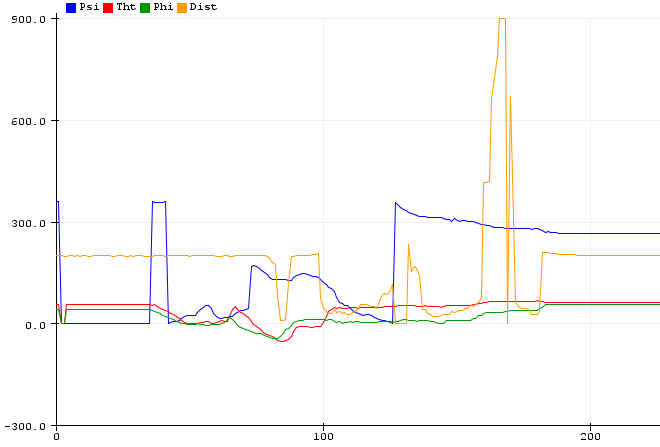
\includegraphics[width=0.7\textwidth]{./Images/serial-plotter.png}
	\caption{\label{fig:serial-plot}Euler Angles and LiDAR Distance Plot Test}
\end{figure}

\subsubsection{Range Reading Harmonization}
\noindent There are more outputs the inertial measurement unit can provide besides the angles. One of most interesting ones is the accelerations. This would be the rate that the velocity of the rollator body is changing with respect to time. 

\noindent This is also where an estimator is useful.\\

\subsubsection{I2C Bus for Sensors}
\noindent The utilization of four ultrasonic sensors and one LiDAR to supply a feed of information to FORWARD's central processor can be integrated and realized through a wiring bus with the I2C digital communication protocol. This I2C scheme will use a synchronous clock signal provided to the sensors by the MCU. It will operate always in half-duplex, meaning data will be transmitted in only one direction at a time - from the MCU to the sensors and from the sensors back to the MCU in successive time steps. Additionally, the sensors will be accessed by their unique addresses and send packets of information as a sequence, taking turns.\\